\documentclass[a4paper]{jreport}	% 日本語の場合

\usepackage{masterThesisJa-Ja}
\usepackage[dvipdfmx]{graphicx}
\usepackage{hyperref}
\usepackage{breakurl}
\pagestyle{empty}
\usepackage{algorithmic}
\usepackage{algorithm}

\setcounter{tocdepth}{3}
\setcounter{page}{-1}

% 【必須】主題:\maintatile{日本語}{英語}
\maintitle{TFライブラリの高性能化とデータ一貫性の確保}{Consistent and scalable TF library}

% 【任意】副題:\subtitle{日本語}{英語}
% 副題が不要な場合は次の行をコメントアウトしてください
%\subtitle{}{}

% 【必須】発表年月:\publish{年}{月}
\publish{2022}{1}

% 【必須】学生情報:\student{学籍番号/CNSアカウント}{氏名(日本語:氏名の間は1文字空ける)}{氏名(英語:Twins登録の表記)}
\student{71970013 / t19501yo}{荻原 湧志}{Yushi Ogiwara}

% 【必須】概要:\abst{概要}
\abst{
 Robot Operating System(ROS)はロボットソフトウェア用のミドルウェアソフトプラットフォームであり、近年多くの研究用ロボットで用いられている。TFライブラリはROSで頻繁に使用されるパッケージであり、ロボットシステム内の座標変換を追跡し、データを変換する標準的な方法を提供するために設計されたものである。ROSの開発初期には複数の座標変換の管理が開発者共通の悩みの種であると認識されていた。このタスクは複雑なために、開発者がデータに不適切な変換を適用した場合にバグが発生しやすい場所となっていた。また、この問題は異なる座標系同士の変換に関する情報が分散していることが多いことが課題となっていた。そこで、TFライブラリは各座標系間の変換を有向森構造として管理し、効率的な座標変換情報の登録、座標変換の計算を可能にした。しかしながら、この有向森構造にはデータの暗黙的な線形補間による一貫性の欠落、及び非効率な並行性制御によりアクセスするスレッドが増えるに従ってパフォーマンスが低下するという問題があることがわかった。そこで、我々はデータベースのトランザクション技術における再粒度ロッキング法、及び並行性制御のアルゴリズムの一種である2PLを応用することにより、この問題を解決した。提案手法では、スレッド数が12までスケールアップすることを示した。また、多くのアクセスパターンにおいて提案手法は既存手法より高いスループットを出すことを示した。
}

% 【必須】研究指導教員(氏名の間は1文字空ける):\advisors{主研究指導教員}{副研究指導教員}
%\advisors{川島 英之}{}
\advisors{川島 英之}


% 以下,本文を出力
\begin{document}

\makecover

\addtolength{\textheight}{-5mm}	% 本文の下限を5mm上昇
\setlength{\footskip}{15mm}	% フッタの高さを15mmに設定
\fontsize{11pt}{15pt}\selectfont

% 目次・表目次を出力
\pagebreak\setcounter{page}{1}
\pagenumbering{roman} % I, II, III, IV
\pagestyle{plain}
\tableofcontents
\listoffigures

% 本文
\parindent=1zw	% インデントを1文字分に設定
\pagebreak\setcounter{page}{1}
\pagenumbering{arabic} % 1,2,3
\pagestyle{plain}

% 章:\chapter{}
% 節:\section{}
% 項:\subsection{}

% 図表:
% \begin{figure}[h]
% \centering
% \begin{center}
% \includegraphics[width=10cm]{fig/<file name>}
% \caption{ <図の一言説明> }\label{fig001}
% \end{center}
% \end{figure}


\chapter{はじめに}
% プレースホルダ
\section{研究背景}

% 質問をここに書く
% abstractでは\citeは使わない?
% 起承転結が二つ?
% 原文から引用しても良いのか?
% ~の問題がある、は喧嘩腰だろうか?
% 面倒なので、有向木と言ってしまう?


% ここもTFの冒頭からコピー
ロボットを使って作業を行う場合、ロボット自身がどこにいるのか、ロボットにはどこにどんなセンサーがついており、また周りの環境のどこにどんなものがあるかをシステムが把握することが重要である。例えば、図\ref{fig:room} のように部屋の中にロボットと、ロボットから観測できる二つの物体があるケースを考える。図中にてロボットは円形、物体は星形で表現される。ロボットが向いている方向は円の中心から円の弧へつながる直線の方向で表している。途中で交わる二つの矢印は各座標系の位置と原点、姿勢を表す。ここでは、地図座標系、ロボットの座標系、二つの物体それぞれの座標系が示されている。

システムはロボットに搭載されたセンサーからのデータを元に各座標系間の位置関係を随時更新する。座標系間の位置関係は並行移動成分と回転成分で表現できる。例えば、自己位置推定プログラムはLiDARから点群データが送られてくるたびにそれを地図データと比較して自己位置を計算し、ロボットが地図座標系にてどの座標に位置するか、ロボットがどの方向を向いているかといった、地図座標系からロボット座標系への位置関係を更新する。物体認識プログラムはカメラからの画像データが送られてくるたびに画像中の物体の位置を計算し、ロボット座標系から物体座標系への位置関係を更新する。

このように、各座標系間の位置関係の更新にはそれぞれ異なるセンサー、プログラムが使われる。各センサーの計測周期、及び各プログラムの制御周期は異なるため、各座標系間の位置関係の更新頻度も異なるものとなる。図\ref{fig:sensor-sync}では、地図座標系からロボット座標系への位置関係データと、ロボット座標系から物体座標系への位置関係データがそれぞれ異なるタイミングで登録されていることを示している。

% SSMはsensor -> osの話で、ROSではosにもう入っていることが前提なのでちょっと話が違うか?


\begin{figure}[h] 
\centering{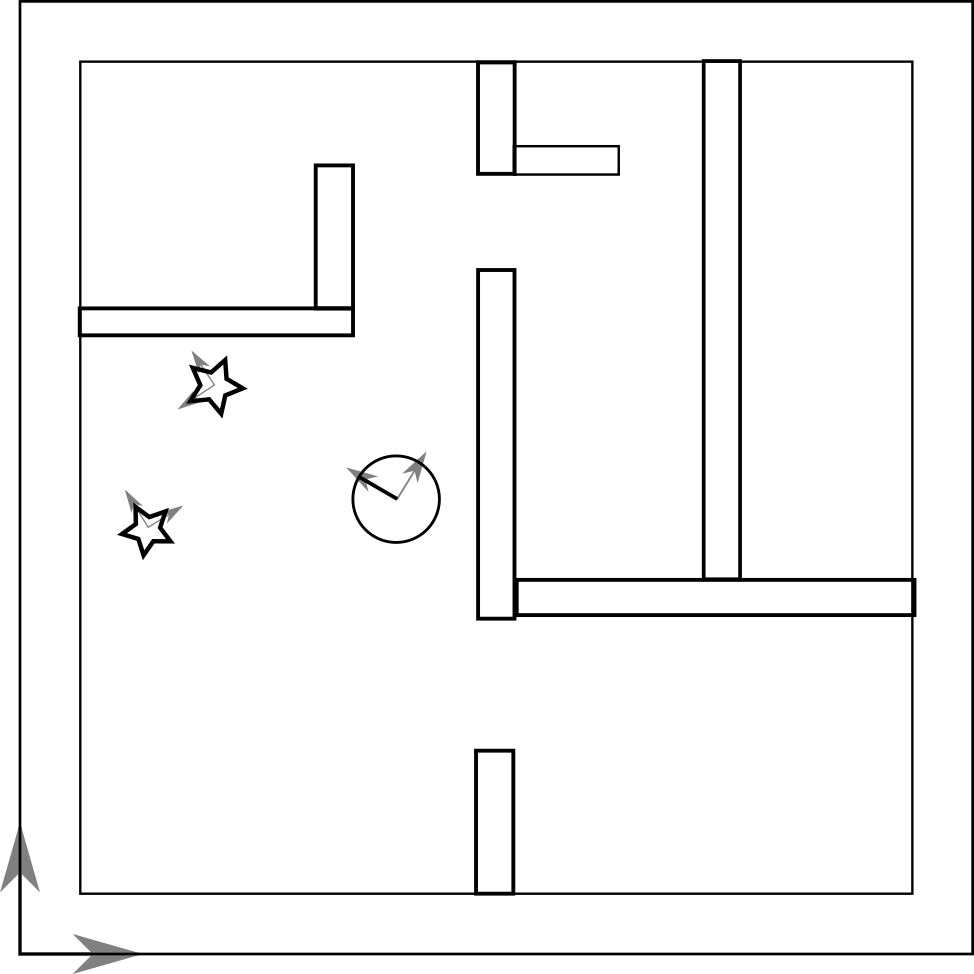
\includegraphics[width=8cm]{room}}	
\caption{部屋の中のロボット}
\label{fig:room}
\end{figure}

\begin{figure}[h] 
\centering{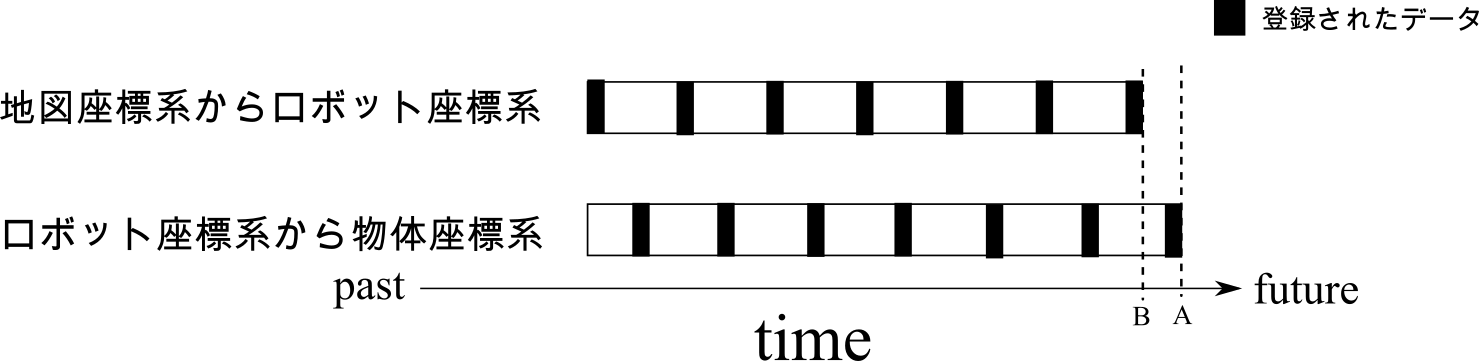
\includegraphics[width=10cm]{sensor-sync}}	
\caption{位置関係の登録のタイムライン}
\label{fig:sensor-sync}
\end{figure}


ここで地図中での物体の位置を把握するために、地図座標系から物体座標系への位置関係を取得する方法について考える。地図座標系から物体座標系への位置関係は地図座標系からロボット座標系への変換とロボット座標系から物体座標系への変換を掛け合わせれば計算ができるが、図\ref{fig:sensor-sync}のように各変換データは異なるタイミングで来るため、最新の変換データを取得するプログラムは複雑なものとなる。Aの時刻で地図座標系から物体座標系への変換データを計算しようとするとロボット座標系から物体座標系への最新の変換データを取得できるが、地図座標系からロボット座標系への変換データはまだ取得できない。このため、最新の変換データ$\theta$を取得する、もしくは過去のデータを元にデータの補外をすると必要がある。Bの時刻で地図座標系から物体座標系への変換データを計算しようとすると地図座標系からロボット座標系への最新の変換データを取得できるが、ロボット座標系から物体座標系への変換データはその時間には提供されていない。このため、$\alpha$と$\beta$のデータから線形補間を行う、もしくは最新の変換データ$\beta$を取得する必要がある。
また、地図座標系からロボット座標系への変換とロボット座標系から物体座標系への変換は別のプログラムで管理されており、座標系同士の変換に関する情報が分散している。

このように、ROSの開発初期には複数の座標変換の管理が開発者共通の悩みの種であると認識されていた。このタスクは複雑なために、開発者がデータに不適切な変換を適用した場合にバグが発生しやすい場所となっていた。また、この問題は異なる座標系同士の変換に関する情報が分散していることが多いことが課題となっていた。

そこで、TFライブラリは各座標系間の変換を有向森構造として一元管理し、効率的な座標系間の変換情報の登録、座標系間の変換の計算を可能にした。まず、図\ref{fig:room}を表す木構造は図\ref{fig:room-tree}で表現できる。木構造のノードが各座標系を表し、木構造のエッジは子ノードから親ノードへの変換データが存在することを表す。
% camera1, camera2の説明はいるだろうか?

\begin{figure}[h] 
\centering
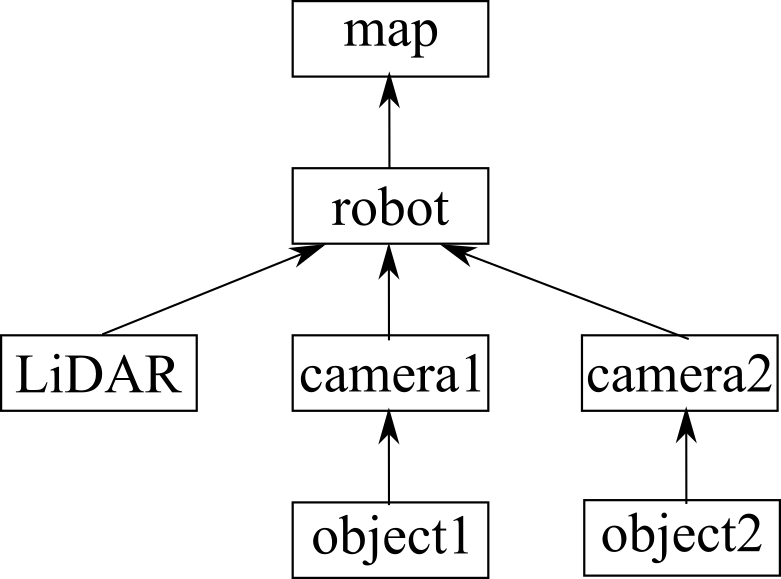
\includegraphics[width=10cm]{tree}	
\caption{図\ref{fig:room}に対応する木構造}
\label{fig:room-tree}
\end{figure}

各ノードはTFではフレームと呼ばれ、ノード中の文字列は各座標系に対応するフレーム名が書かれている。図\ref{fig:room-tree}では地図座標系のフレーム名はmap、ロボット座標系のフレーム名はrobot、物体1の座標系のフレーム名はobject1となる。木構造は子ノードから親ノードへポインタが貼られ、子ノードから親ノードを辿ることができる。このため、mapからobject1への座標変換を計算するにはobject1からmapへの座標変換の計算し、その逆数を取る必要がある。

子ノードから親ノードへの位置関係は子ノードが保持する。図中では示されていないが、木のルートノードのエッジはNULLポインタを指している。

先程説明したように、各フレーム間の座標変換情報はそれぞれ異なるタイミングで登録される。これに対処するため、TFでは各フレーム間の座標変換情報を過去一定期間保存する。図\ref{fig:room-tree}において各フレーム間の座標変換情報が登録されたタイミングを表すのが図\ref{fig:room-timeline}である。横軸は時間軸を表し、左側が過去、右側が最新の時刻を表す。黒色のセルはデータがその時刻にデータが登録されたことを表す。時刻Aではrobotからmapへの座標変換の情報が得られるが、object1からmapへの座標変換の情報は時刻Aには存在しない。そこで、TFでは前後のデータから線形補間を行うことにより該当する時刻の座標変換データを計算する。つまり、TFは該当する時刻の座標変換データが保存されている、もしくは前後の値を元に線形補間ができる場合にはその時刻の座標変換データを提供できる、とみなす。灰色の領域は線形補間により座標変換データが提供可能な時間領域を表す。

\begin{figure}[h] 
\centering
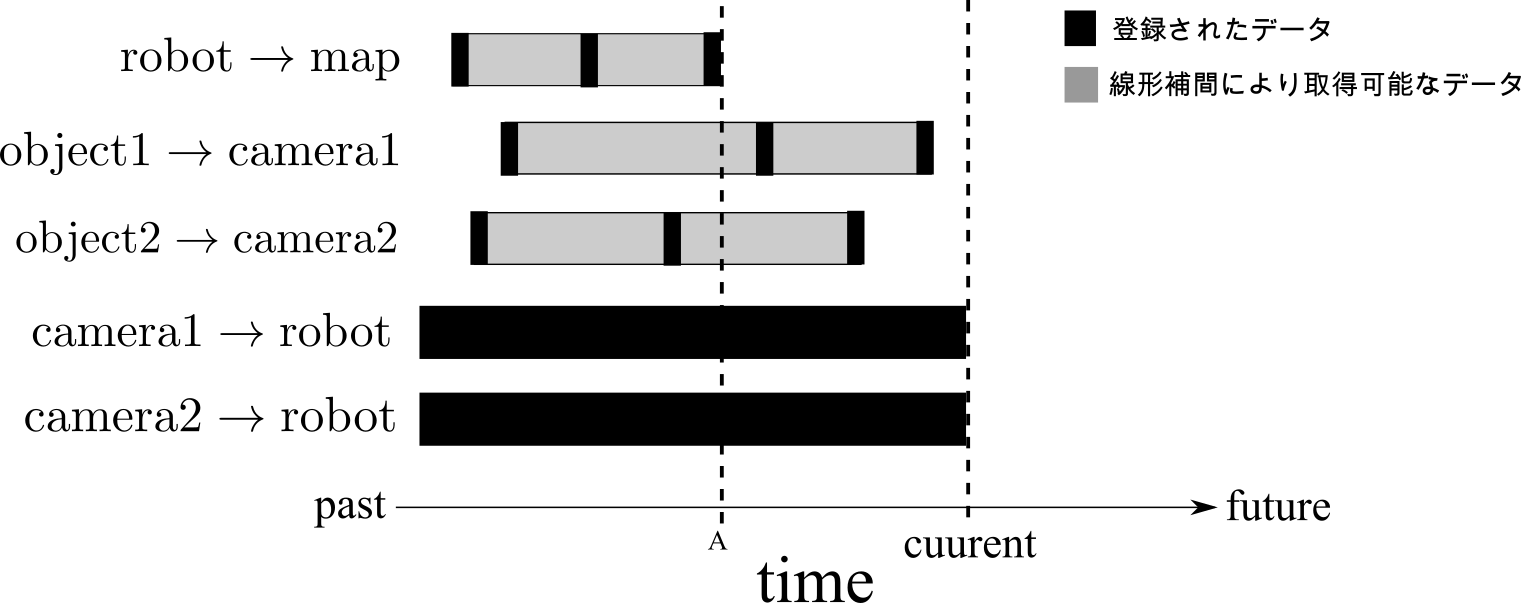
\includegraphics[width=10cm]{room-timeline}	
\caption{図\ref{fig:room-tree}における位置関係登録のタイムライン}
\label{fig:room-timeline}
\end{figure}

図\ref{fig:room-tree}における位置関係登録のタイムラインが図\ref{fig:room-timeline}のようになっているとき、TFではobject1からmapへの最新の位置関係は次のように計算する。

まず、object1からmapへのパスを確認する。ここではobject1からmapへのパスは$object1 \rightarrow camera1$, $camera1 \rightarrow robot$, $robot \rightarrow map$であることがわかる。

次に、どのパスにおいてもなるべく最新の座標変換を提供できる時刻を確認する。図\ref{fig:room-timeline}を確認すると、$object1 \rightarrow camera1$, $camera1 \rightarrow robot$, $robot \rightarrow map$において最新の座標変換情報が登録された時刻が最も古いのは$robot \rightarrow map$である。このため、時刻Aがここでは要件を満たす。

最後に、時刻Aでの各パスのデータを取得し、それらを掛け合わせる。$robot \rightarrow map$については登録されたデータを使い、$object1 \rightarrow camera1$, $camera1 \rightarrow robot$については線形補間によってデータを取得する。

\section{研究課題}
前述したようにTFはロボットシステム内部の座標系間の位置関係を一元管理する機構を提供する。しかしながら、これには以下のような問題点が挙げられる。

\subsection*{問題1:ジャイアント・ロック}
TFの森構造には複数のスレッドがアクセスするため並行性制御が必要となるが、既存のTFでは一つのスレッドが森構造にアクセスしている際は他のスレッドは森構造にアクセスできないアルゴリズムとなっている。これは、マルチコアが常識となっている現代では大きな問題となる。

\subsection*{問題2:データの一貫性}

上記の説明のように、TFのフレーム間の座標変換計算インターフェースは最新のデータを使わない可能性がある。そこで、最新のデータを取得できるインターフェースを追加する。

\section{研究方針}
前述した問題1については、データベースの並行性制御技術における細粒度ロッキング法を適用して解決する。細粒度ロッキング法は、並行性制御においてロックするデータの単位をなるべく小さくし、並行性を向上させる手法である。問題2については、データベースのトランザクション技術における2PLを適用した新たなインターフェースを提供することにより解決する。2PLとは、複数のデータに対するロック・アンロックのタイミングを二つのフェーズに分けることにより並行性を向上させつつデータ操作の一貫性を確保する手法である。

\section{貢献}

本研究ではデータベースのトランザクション技術における再粒度ロッキング法、及び並行性制アルゴリズムの一種である2PLを応用することにより、問題1および問題2を解決した。

\section{構成}
本論文の構成は次の通りである。第二章では関連研究について述べる。第三章では既存のTFの森構造とその問題点について述べる。第四章では提案手法である森構造への再粒度ロックの導入とデータ一貫性のためのインターフェイスの提供について述べる。第五章では提案手法の評価結果を述べる。第六章では本研究の結論を述べる。第七章では今後の課題について述べる。

\chapter{関連研究}
データベース分野におけるロボットの研究の例としてGAIA platform\cite{gaia}が挙げられる。


TFのようにデータを時系列的に管理するものとしてSSMが挙げられる。
% 移動ロボット用センサ情報処理ミドルウェアの開発 か?


データベースの技術をロボットに適用するという内容ではGAIA\cite{gaia}が挙げられる。
ロボットというより自律システム

C++に宣言的にデータ変更時のルールを記述できる。これによって簡単にイベントベース
trigger付きのUDFみたいな?

これはRDBベースでreactiveな挙動を提供する。


プロダクトレベルのものを目指すROS2\cite{ros2}やAutoware\cite{autoware}でも、livelinessなどの指標
DDS
が導入されたが、データベースの並行性制御の導入はない。



本研究のようなアプローチは存在しない。


2PL以外の並行性制御アルゴリズムとしてはSilo\cite{silo}が挙げられる。

% ここは後で書こうっと


\chapter{既存のTF森の構造とその問題点}
%TF森の実態はtf2パッケージ中にあるBufferCoreクラス\cite{buffer-core} である。
\section{構造}
TFライブラリでは図\ref{fig:multitree} のように各座標系間の位置関係を森構造で管理し、複数の木の登録が登録できる。ノードが各座標系を表し、エッジは子ノードから親ノードへの座標変換データが存在することを表す。各ノードはフレームと呼ばれ、ノード内の文字列は各座標系に対応するフレーム名が書かれている。

各フレーム間の座標変換情報は過去10秒間保存される。このため、各フレーム間の座標変換情報が登録された時刻を図\ref{fig:general-timeline}のようなタイムラインで表現できる。黒のセルは登録されたデータを表し、灰色のセルは線形補間により座標変換データが取得可能な時刻を表す。横軸が時間軸を表し、左側が過去、右側が最新の時刻を表す。



\begin{figure}[h] 
\centering
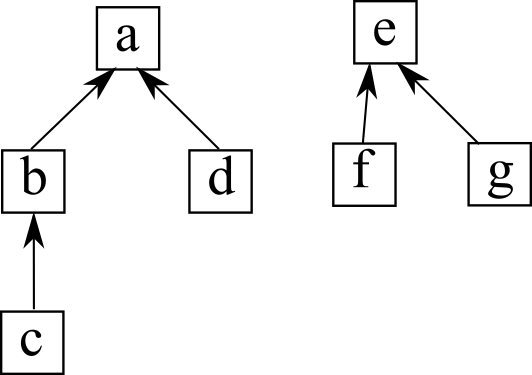
\includegraphics[width=7cm]{multitree.png}	
\caption{複数の木構造}
\label{fig:multitree}
\end{figure}

\begin{figure}[h] 
\centering
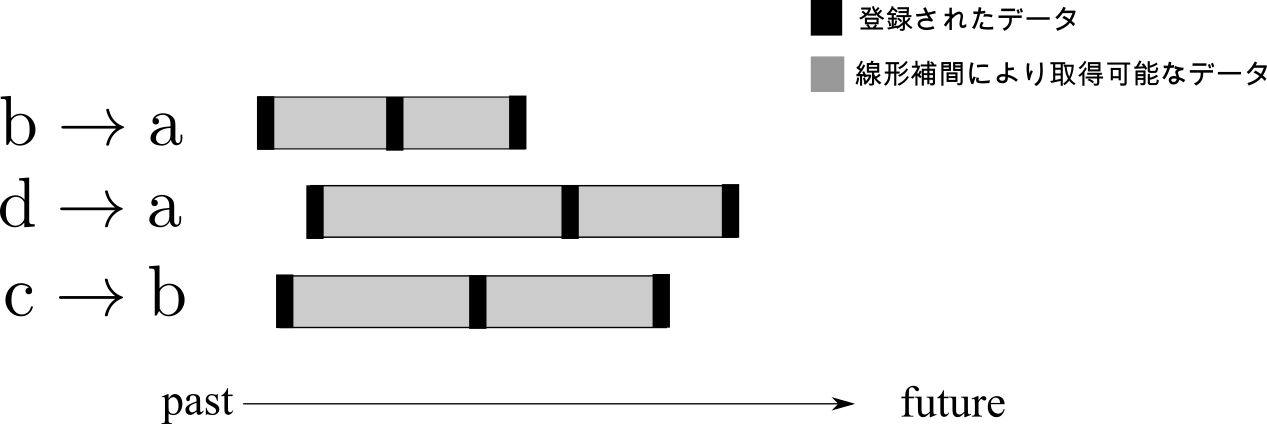
\includegraphics[width=10cm]{general-timeline.png}
\caption{タイムライン}
\label{fig:general-timeline}
\end{figure}


\section{lookupTransform}
二つのフレーム間の座標変換情報を取得するにはlookupTransformメソッドを使う。

登録されたフレームが図\ref{fig:multitree}、登録された座標変換情報のタイムラインが図\ref{fig:general-timeline}の状況において、lookupTransformメソッドを用いてフレームcからフレームdへの座標変換を計算するアルゴリズムを説明する。

\begin{enumerate}
	\item フレームcから木構造のルートノードへのパスを取得する。ここではルートノードはaとなり、フレームcからフレームaへのパスはc$\rightarrow$bとb$\rightarrow$aとなる。
	\item フレームdから木構造のルートノードへのパスを取得する。同じようにルートノードはaとなり、フレームdからフレームaへのパスはd$\rightarrow$aとなる。
	\item 得られた三つのどのパスにおいてもなるべく最新の座標変換を提供できる時刻を確認する。ここでは時刻Aが要件を満たす。
	\item 時刻Aにおける各パスの座標変換データを計算する。b$\rightarrow$aについては登録されたデータを利用でき、c$\rightarrow$bとd$\rightarrow$aについては線形補間されたデータを利用できる。
	\item 最後に、フレームcからフレームaへの座標変換と、フレームaからdへの座標変換を掛け合わせる。フレームcからフレームaへの座標変換はc$\rightarrow$bとb$\rightarrow$aの
\end{enumerate}



最後に、フレームcからフレームaへの座標変換と、フレームaからdへの座標変換を掛け合わせる。フレームcからフレームaへの座標変換はc$\rightarrow$bとb$\rightarrow$aの

% ショートカットについては説明不要?


例外パターンの説明

また、lookupTransformは指定した時刻のデータを取得することもできる。



擬似コード

\begin{algorithm}[H]
	\caption{lookupTransform}
	\begin{algorithmic}
	\STATE e = walkToTopParent
	\IF{$n < 0$}
	\STATE $X \leftarrow 1 / x$
    \STATE $N \leftarrow -n$
    \ENDIF
	\end{algorithmic}
\end{algorithm}


まずはrunning exampleを示す。なるべくC++レベルでの説明は避けるべきか。
とりあえず、途中で親が変わらないと仮定する。じゃないと説明が面倒

1. sourceからrootへの座標変換を計算
2. targetからrootへの座標変換を計算
3. sourceからrootへの座標変換 * rootからtargetへの座標変換を計算

まずは普通のケースから。同じ親を持ち、
%    r
%   / \
%  /   \
%  a     c
% / \
% b e
%/
%d
%
% d -> e
まずはこの時間で見ていく
まずはdからrへの座標変換を計算
次にeからrへの座標変換を計算
rからeへの座標変換は、単にeからrへの逆変換をとれば良い。
あとはdからrへの変換 * rからeへの変換で計算できる

% r
% |
% t
% |
% s

このようにtargetが直接の

ここら辺は説明省いても良い????

この例のように、sourceとtargetが同じ木の中にない場合、つまり同じrootを共有しない場合にはエラーとなる。


running exampleが十分であれば、擬似アルゴリズムでの説明を省けるかも。

\begin{algorithm}[H]
	\caption{walkToTopParent(time, source\_id, target\_id)}
	\begin{algorithmic}
	\STATE frame\_id = source\_id
	\STATE top\_parent\_id = frame\_id
	\STATE // source frameからrootへのパスをたどる
	\WHILE{ frame\_id $\neq$ 0 }
	\STATE cache = getFrame(frame\_id)
	\IF{cache = NULL}
	\STATE // 木構造のrootに到達
	\STATE top\_parent\_id = frame\_id
	\STATE \textbf{break}
	\ENDIF
	\STATE paret\_id = cacheから座標変換と親のidを取得
	\IF{frame\_id == target\_id }
	\STATE // target frameはsource frameの祖先なので早期リターン
	\STATE 累積したデータから座標変換を計算
	\RETURN 0
	\ENDIF
	\STATE 座標変換を蓄積
	\STATE top\_parent\_id = frame\_id
	\STATE frame\_id = parent\_id
	\ENDWHILE
	
	\STATE // target\_idからrootへのパスをたどる
	\STATE frame\_id = target\_id
	\WHILE{ frame\_id $\neq$ top\_parent\_id }
	\STATE cache = getFrame(frame\_id)
	\IF{cache = NULL}
	\STATE // 木構造のrootに到達
	\STATE \textbf{break}
	\ENDIF
	\STATE parent\_id = cacheから座標変換と親のidを取得
	\IF{frame\_id == source\_id }
	\STATE // source frameはtarget frameの祖先なので早期リターン
	\STATE 累積したデータから座標変換を計算
	\RETURN 0
	\ENDIF
	\STATE 座標変換を蓄積
	\STATE frame\_id = parent\_id
	\ENDWHILE
	\IF{frame\_id $\neq$ top\_parent\_id}
	\STATE // source frameとtarget frameは同じ木構造に属していない
	\RETURN エラーコード
	\ENDIF
	\STATE // source frameとtarget frameは祖先関係にはないが、同じ木に属している
	\STATE source frameからtarget frameへの座標変換の計算
	\RETURN 0
	\end{algorithmic}
\end{algorithm}




\section{setTransform}

座標変換を登録する。特に説明の必要はない


\section{問題点}

ここより上の部分では、どの程度エラーケースを、どの程度正確な説明が必要か不明瞭。とりあえず以下を書き下す。

giant lock

最新のデータを返さない
exampleを示そう
%
% a  |  | |
% b    | 
% c   | | 
この場合には、bに引っ張られてaの最新のデータが取れない

線形補間により、一貫性がないケースがある。
例えば関節間の制約やジンバルロック、特異点など
制御プログラムが意図しない状態を見てしまうかもしれない

\chapter{提案手法}

まず、ginat lockをしない方法を導入
読み書きを行う際には必要なノードのみlockする

setTransformとは異なり、lookupTransformは各ノードの情報の読み込みのみ行う。

読み込み処理であれば複数のスレッドからの同時アクセスを行ってもdata raceは発生しない。このため、


S lockはdata raceが発生しないreadの時に、X lockは二つ以上のスレッドからwrite操作されるとdata raceが発生するのを防ぐために使われる。

(S-Xはもう古い?readとwriteの方が説明が適切?)


さらに、shared lockとexclusive lockを導入する
これは次のような表で表現できる
%   N | S | X
% S o   o   x   
% X o   x   x
%
表は列が既にかかっているロック(Nは何もかかっていない)、行はかけようとしているロックを表し、oであれば新たにかけようとしているロックの確保に成功し、xであればロックがかけられないことを表す
例えば、S lockが既にかけられていても新たにS lockを他のスレッドが書けることが可能になる。対し、X lockが既にかかっている場合にはS lockはかけられず、S lockがかかっている場合にもX lockはかけられない。X lockをかけることができるスレッドは常に一つだけである。


続いて、最新のデータを取らない問題と線形補間によりデータの一貫性がなくなる問題について

既存のlookupTransformでは、最新のデータを取得しようとしても過去のデータを参照してしまう、また線形補間されてしまう

最新のデータをそれぞれ取ってくるという方法もサポートする。(しかしこれだけでは十分ではない。 <- この導入はいまいち。)冒頭で説明したように、ROSは分散アーキテクチャを採用する。TFMessageには各フレーム間の座標変換情報を複数登録できるが、TFは複数の座標変換をsetTransformを複数回呼び出すことにより実現している。これにより、中間の状態を見てしまう。これは図のように説明できる。
この図のように、giant lockを毎回のsetTransformで取ってはいるが、その操作が終わり次のsetTransformsを呼ぶまでの間はlockが外される。これにより、一貫性のない状態を見てしまう恐れがある。


そこで、我々は最新のデータをatomicに取得するlookupLatestTransform、及び複数の座標変換を一度にatomicに登録できるseTransformsを追加した。複数のデータに対する読み込み、書き込みをatomicに行うために、我々は2PL[?]を実装した。

しかしながら2PLにはdead lockの問題がある。
例えば次の例、これは木を登る方向と下る方向の両方があるからこうなる。

データをreorderできれば2PLではdeadlockは発生しない(DAGが構築できる)、がTF木ではできそうにない。

そこで我々はdeadlock preventの方法としてNo-wait[Bern 1981]を採用した。これはwrite lockをかけようとして失敗したら最初からやり直す。

Wound wait, nonpreemptive (Concurrency Control in Distributed Database Systems PHLIP.A BERNSTEIN AND NATHAN GOODMAN P196)

transactionにpriorityを足すとかは?



\chapter{評価}
実験を行う

スレッド数を上げるとスループット伸びる
jointを増やすと緩やかにスループットが落ちる
iterを増やすと1000以降で急激にスループットが下がる。no waitによる弊害か?lockの確保に失敗しているのかも
read ratioは高くなるほどブロックされる可能性が減る
read lenは安定しているように見える。なぜtrnでread lenが小さいとこうなるのか。。。2PLでロックする箇所が変わるから?

write lenを上げるとやはりブロックされる部分が増える



\chapter{結論}
再粒度ロックの導入により、パフォーマンスを上げることができた
特に、スレッド数の増加とともにスループットが下がる問題を解決できた

データの一貫性は必須、というデータも示したい。

\chapter{今後の課題}
ここでは取り上げなかったTF木の問題点として、部分的に座標情報の登録に失敗するケース。rollbackなどもいれtransactionalに行う必要

また、insert/deleteが大量に発生するケースも考える。


\chapter*{謝辞}
\addcontentsline{toc}{chapter}{\numberline{}謝辞}

本研究を進めるにあたり、慶應義塾大学准教授川島英之先生とサイボウズラボ株式会社星野喬様に頂きました優れた御指導により、私の研究はとても有意義で満ち足りたものとなりました。また、慶應義塾大学川島研究会秘書藤川綾様には幾多の手続きを丁寧にサポートして頂き,円滑な出張や書類作成,研究環境整備を行うことができました。そして、CCBench開発者である株式会社ノーチラス・テクノロジーズ田辺敬之様。この研究に関わっていただいたすべての方に深く感謝を申し上げます。

% 参考文献(References)
\newpage
\addcontentsline{toc}{chapter}{\numberline{}参考文献}
\renewcommand{\bibname}{参考文献}



%% 参考文献に bibtex を使う場合
%\bibliographystyle{junsrt}
%\bibliography{ref}

%% 参考文献を直接ファイルに含めて書く場合
	
\begin{thebibliography}{99}


\bibitem{ros} M. Quigley, K. Conley, B. P. Gerkey, J. Faust, T. Foote, J. Leibs, R. Wheeler, and A. Y. Ng, “Ros: an open-source robot operating system,” in ICRA Workshop on Open Source Software, 2009.

\bibitem{tf} T. Foote, "tf: The transform library," 2013 IEEE Conference on Technologies for Practical Robot Applications (TePRA), 2013, pp. 1-6, doi: 10.1109/TePRA.2013.6556373.

\bibitem{2PL} Philip A. Bernstein and Nathan Goodman, "Concurrency Control in Distributed Database Systems" in ACM Computing Surveys, 1981, pp. 185-221

\bibitem{buffer-core} "BufferCore.h", \url{https://github.com/ros/geometry2/blob/noetic-devel/tf2/include/tf2/buffer_core.h}

\bibitem{gaia} "GAIA platform", \url{https://www.gaiaplatform.io}

\bibitem{ros2} "ROS2", \url{https://docs.ros.org/en/rolling/}

\bibitem{autoware} "Autoware", \url{https://tier4.jp/en/autoware/}

\bibitem{silo} Stephen Tu, Wenting Zheng, Eddie Kohler †, Barbara Liskov,
and Samuel Madden. Speedy transactions in multicore in-memory
databases. In SOSP, pages 18–32. ACM, 2013

\end{thebibliography}


\end{document}
